\documentclass[man, fleqn, noextraspace]{apa6}
\usepackage{lmodern}
\usepackage{amssymb,amsmath}
\usepackage{ifxetex,ifluatex}
\usepackage{fixltx2e} % provides \textsubscript
\ifnum 0\ifxetex 1\fi\ifluatex 1\fi=0 % if pdftex
  \usepackage[T1]{fontenc}
  \usepackage[utf8]{inputenc}
\else % if luatex or xelatex
  \ifxetex
    \usepackage{mathspec}
  \else
    \usepackage{fontspec}
  \fi
  \defaultfontfeatures{Ligatures=TeX,Scale=MatchLowercase}
\fi
% use upquote if available, for straight quotes in verbatim environments
\IfFileExists{upquote.sty}{\usepackage{upquote}}{}
% use microtype if available
\IfFileExists{microtype.sty}{%
\usepackage{microtype}
\UseMicrotypeSet[protrusion]{basicmath} % disable protrusion for tt fonts
}{}
\usepackage{hyperref}
\hypersetup{unicode=true,
            pdftitle={Lab9-Heidi-Jeongim-Jungah},
            pdfauthor={Jungah-Lee, Jeongim Jin, \& Heidi Shi},
            pdfkeywords={Community of Practice, Language Socialization},
            pdfborder={0 0 0},
            breaklinks=true}
\urlstyle{same}  % don't use monospace font for urls
\usepackage{graphicx,grffile}
\makeatletter
\def\maxwidth{\ifdim\Gin@nat@width>\linewidth\linewidth\else\Gin@nat@width\fi}
\def\maxheight{\ifdim\Gin@nat@height>\textheight\textheight\else\Gin@nat@height\fi}
\makeatother
% Scale images if necessary, so that they will not overflow the page
% margins by default, and it is still possible to overwrite the defaults
% using explicit options in \includegraphics[width, height, ...]{}
\setkeys{Gin}{width=\maxwidth,height=\maxheight,keepaspectratio}
\IfFileExists{parskip.sty}{%
\usepackage{parskip}
}{% else
\setlength{\parindent}{0pt}
\setlength{\parskip}{6pt plus 2pt minus 1pt}
}
\setlength{\emergencystretch}{3em}  % prevent overfull lines
\providecommand{\tightlist}{%
  \setlength{\itemsep}{0pt}\setlength{\parskip}{0pt}}
\setcounter{secnumdepth}{0}
% Redefines (sub)paragraphs to behave more like sections
\ifx\paragraph\undefined\else
\let\oldparagraph\paragraph
\renewcommand{\paragraph}[1]{\oldparagraph{#1}\mbox{}}
\fi
\ifx\subparagraph\undefined\else
\let\oldsubparagraph\subparagraph
\renewcommand{\subparagraph}[1]{\oldsubparagraph{#1}\mbox{}}
\fi

%%% Use protect on footnotes to avoid problems with footnotes in titles
\let\rmarkdownfootnote\footnote%
\def\footnote{\protect\rmarkdownfootnote}


  \title{Lab9-Heidi-Jeongim-Jungah}
    \author{Jungah-Lee\textsuperscript{1}, Jeongim Jin\textsuperscript{2}, \& Heidi
Shi\textsuperscript{3}}
    \date{}
  
\shorttitle{w5lab9}
\affiliation{
\vspace{0.5cm}
\textsuperscript{1} University of Oregon\\\textsuperscript{2} University of Oregon\\\textsuperscript{3} University of Oregon}
\keywords{Community of Practice, Language Socialization\newline\indent Word count: X}
\usepackage{csquotes}
\usepackage{upgreek}
\captionsetup{font=singlespacing,justification=justified}

\usepackage{longtable}
\usepackage{lscape}
\usepackage{multirow}
\usepackage{tabularx}
\usepackage[flushleft]{threeparttable}
\usepackage{threeparttablex}

\newenvironment{lltable}{\begin{landscape}\begin{center}\begin{ThreePartTable}}{\end{ThreePartTable}\end{center}\end{landscape}}

\makeatletter
\newcommand\LastLTentrywidth{1em}
\newlength\longtablewidth
\setlength{\longtablewidth}{1in}
\newcommand{\getlongtablewidth}{\begingroup \ifcsname LT@\roman{LT@tables}\endcsname \global\longtablewidth=0pt \renewcommand{\LT@entry}[2]{\global\advance\longtablewidth by ##2\relax\gdef\LastLTentrywidth{##2}}\@nameuse{LT@\roman{LT@tables}} \fi \endgroup}


\DeclareDelayedFloatFlavor{ThreePartTable}{table}
\DeclareDelayedFloatFlavor{lltable}{table}
\DeclareDelayedFloatFlavor*{longtable}{table}
\makeatletter
\renewcommand{\efloat@iwrite}[1]{\immediate\expandafter\protected@write\csname efloat@post#1\endcsname{}}
\makeatother
\usepackage{lineno}

\linenumbers

\authornote{Jung-ah Lee joined the Department of East Asian
Langauges and Literatures at the Unviersity of Oregon at 2017.

Correspondence concerning this article should be addressed to
Jungah-Lee, 1248 University of Oregon Eugene, Oregon 97403-1248. E-mail:
\href{mailto:jlee27@uoregon.com}{\nolinkurl{jlee27@uoregon.com}}}

\abstract{
This article provides an introduction to this issue of Language in
Society by exploring the relationship of the concept of Community of
Practice (CofP) to related terms and theoretical frameworks. The
criterial characteristics and constitutive features of a CofP are
examined; the article points out how a CofP framework is distinguished
from other sociolinguistic and social psy- chological frameworks,
including social identity theory, speech community, social network and
social constructionist approaches. (Community of Practice, speech
community, gender, sex, social practice, ethnographic sociolinguistics,
discourse analysis)


}

\begin{document}
\maketitle

{
\setcounter{tocdepth}{4}
\tableofcontents
}
\newpage

\section{\texorpdfstring{\textbf{Methods}}{Methods}}\label{methods}

We adopted the method introduced by Pan and Kádár (2011), the author of
\emph{Phonetics and phonology of Nantong Chinese}We used methods
introduced by Ahmed, Arai, and Attia (2001). Besides we also adopted the
diligent and collaborative approach to Rstudio (see Kádár and Pan
(2011)).

\subsection{\texorpdfstring{\emph{Participants}}{Participants}}\label{participants}

The authors gathered teenagers who attend different schools on the
Pacific Northwest, \emph{Eugene,Oregon}.

\subsubsection{Males}\label{males}

n=4

\subsubsection{Females}\label{females}

n=4

\paragraph{Female Subjects from High School
A}\label{female-subjects-from-high-school-a}

n=2

\paragraph{Female Subjects from High School
B}\label{female-subjects-from-high-school-b}

n=2

\subsection{\texorpdfstring{\emph{Material}}{Material}}\label{material}

\subsection{\texorpdfstring{\emph{Procedure}}{Procedure}}\label{procedure}

\subsection{\texorpdfstring{\emph{Data
analysis}}{Data analysis}}\label{data-analysis}

We used Pan and Kádár (2011) for all our analyses.

\[
math_t2i = \alpha + \beta_1(math_t1i) + \beta_2(SES_cat1) + \beta_3(math_t1i x SES_cat1)\epsilon 
\]

\begin{figure}
\centering
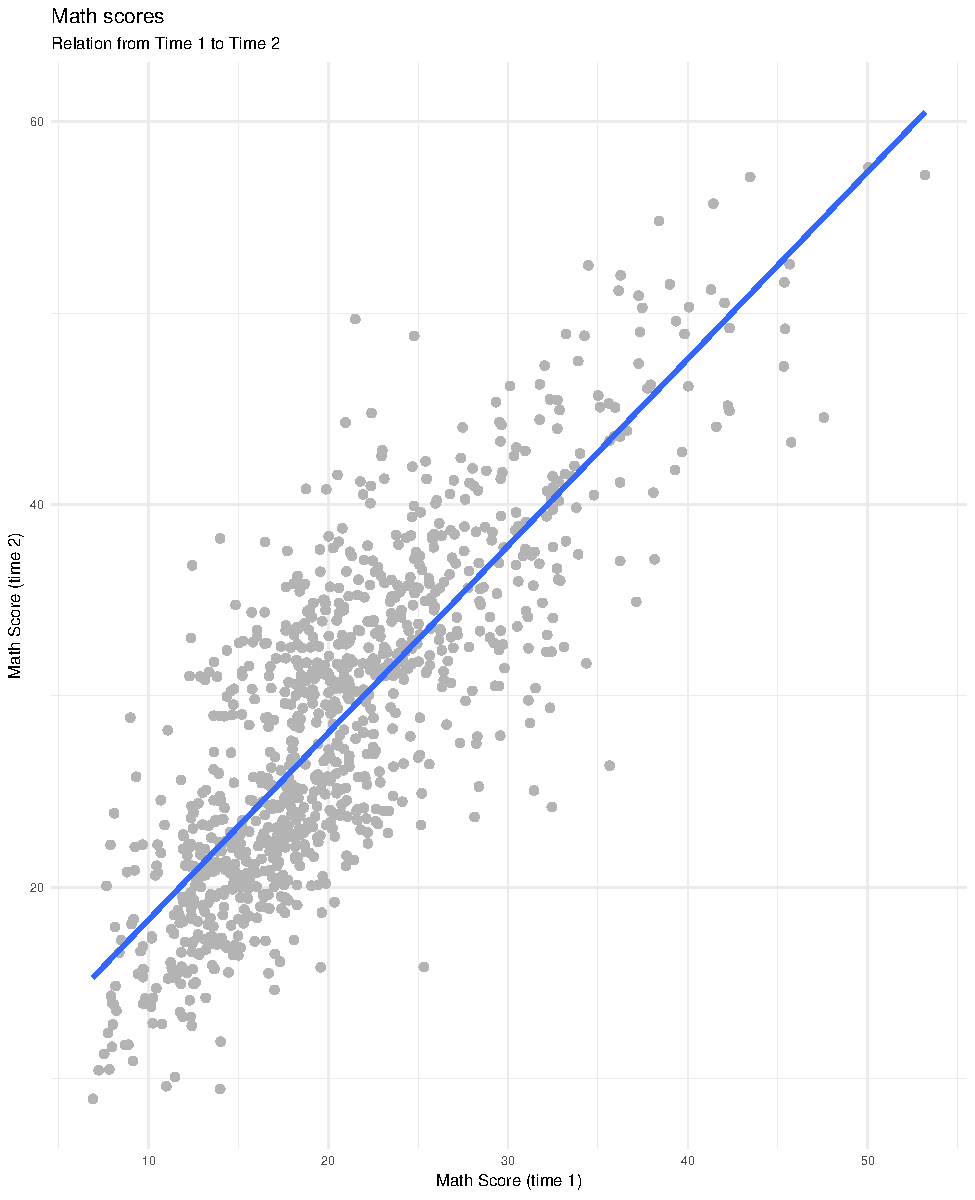
\includegraphics{Lab9-Heidi-Jeongim-Jungah_files/figure-latex/Question5-1.pdf}
\caption{}
\end{figure}

\section{\texorpdfstring{\textbf{Results}}{Results}}\label{results}

Therefore, it is found that the math scores of su

\section{\texorpdfstring{\textbf{Discussion}}{Discussion}}\label{discussion}

\newpage

\section{\texorpdfstring{\textbf{References}}{References}}\label{references}

\begingroup
\setlength{\parindent}{-0.5in} \setlength{\leftskip}{0.5in}

\hypertarget{refs}{}
\hypertarget{ref-ahmed2001}{}
Ahmed, A. H., Arai, S., \& Attia, A. K. (2001). Petrological
characteristics of podiform chromitites and associated peridotites of
the pan african proterozoic ophiolite complexes of egypt.
\emph{Mineralium Deposita}, \emph{36}(1), 72--84.

\hypertarget{ref-kadar2011}{}
Kádár, D. Z., \& Pan, Y. (2011). Politeness in china. \emph{Politeness
in East Asia}, 125--146.

\hypertarget{ref-pan2011}{}
Pan, Y., \& Kádár, D. Z. (2011). \emph{Politeness in historical and
contemporary chinese}. A\&C Black.

\endgroup


\end{document}
